\chapter{Hardware}

\paragraph*{}
Due to the predicted cost of hardware, we decided to ask a local Chulalongkorn University robotics club for one of their swarm robots, particularly the robot used in a previous RoboCup soccer competition. While the electronics in these robots are outdated, the motors remain exceptional, as they are Maxon motors, known for their reliability, efficiency, and speed. Hiveground, one of our project supporters, has also agreed to provide us with another identical robot, as one of the founders is an alumnus of the EIC. At the time of writing, we currently have two identical robots in our possession.
\begin{figure}[H]
    \centering
    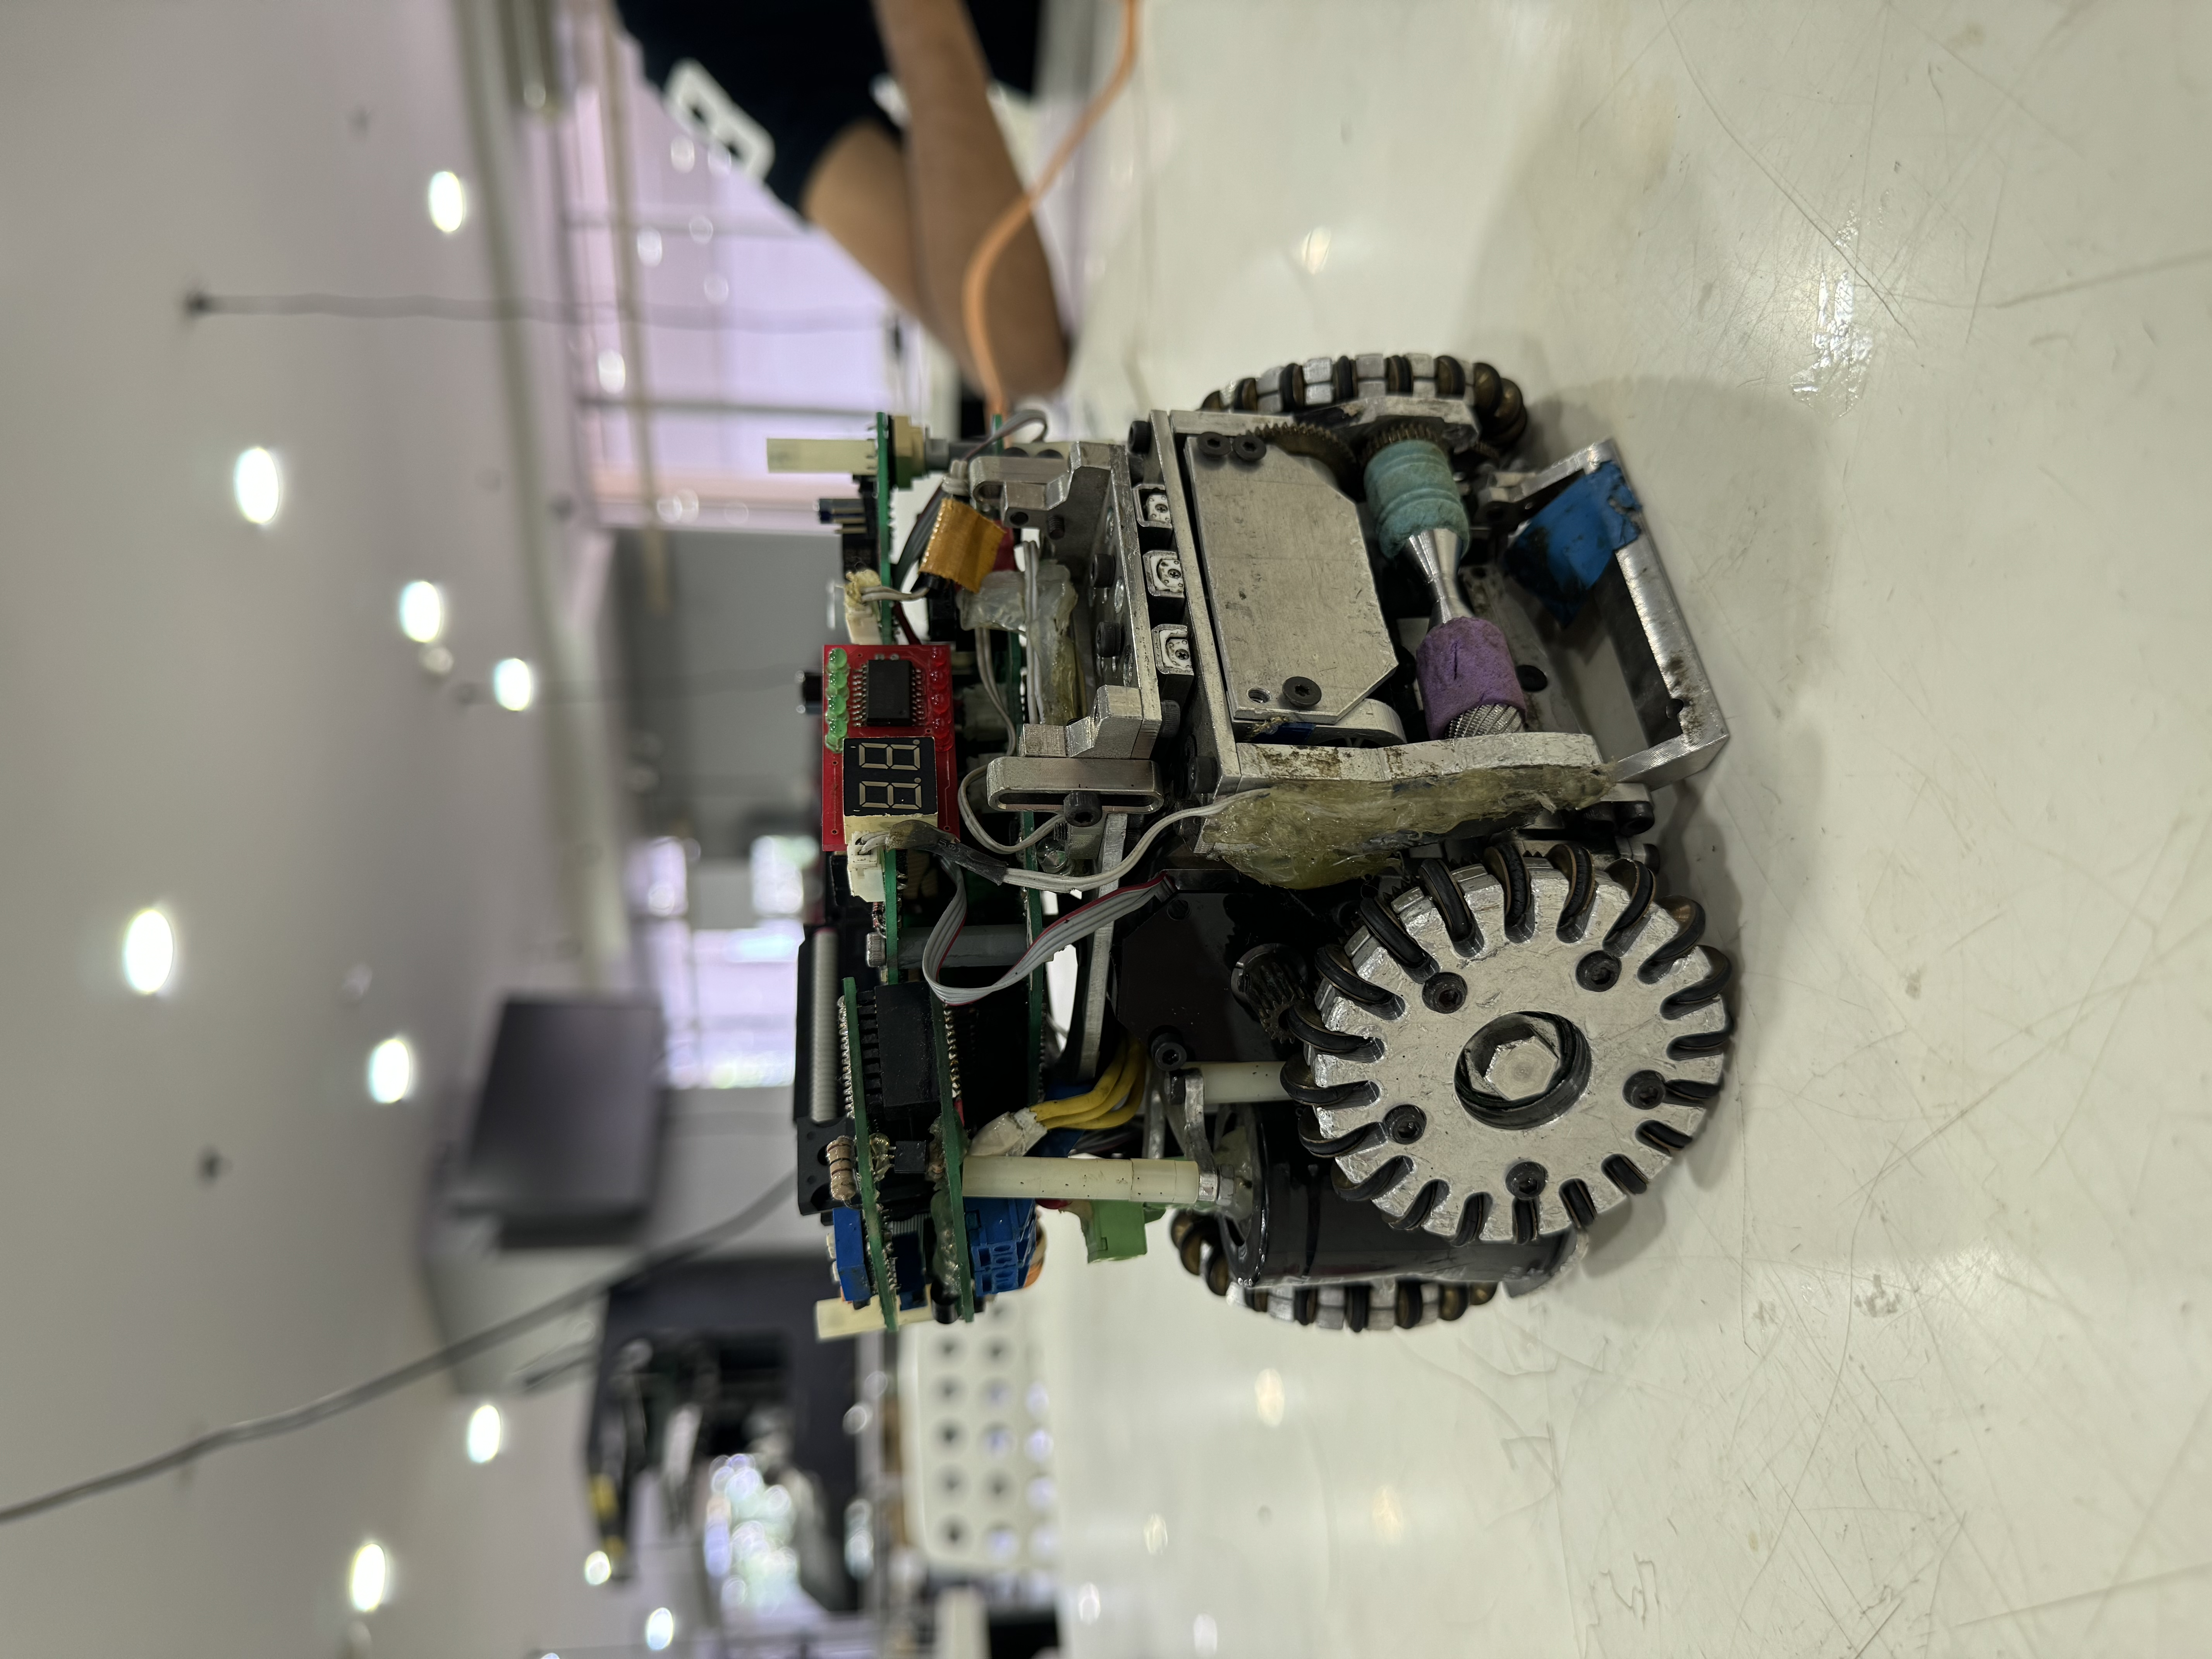
\includegraphics[width=0.4\linewidth, angle=270]{assets/images/hardware/robobot.JPG}
    \caption{One of the robots obtained from EIC Chula, RoboCup}
    \label{fig:robobot}
\end{figure}
\paragraph*{}
The Maxon motors in both robots are arranged in an X layout, paired with high-quality omnidirectional wheels. However, due to a lack of use over the past decade, the rubber on the wheels has decayed. Given the custom nature of these wheels, we will 3D print new rubber O-rings to replace the old ones.
\paragraph*{}
The next step involves testing the motors, including their encoders, to evaluate the accuracy, power, and torque of the current setup. Our goal is to determine whether these motors can perform adequately as servo motors for precise control and calculations. For this purpose, we will use an Arduino to control the motors during testing.
\paragraph*{}
In terms of schedule, we are currently ahead of the planned timeline for the hardware development stage, giving us some flexibility for further testing and refinement.